% !TEX TS-program = pdflatex
% !TEX encoding = UTF-8 Unicode

% This is a simple template for a LaTeX document using the "article" class.
% See "book", "report", "letter" for other types of document.

\documentclass[11pt]{article} % use larger type; default would be 10pt

\usepackage[utf8]{inputenc} % set input encoding (not needed with XeLaTeX)
\usepackage[english]{babel}

%%% Examples of Article customizations
% These packages are optional, depending whether you want the features they provide.
% See the LaTeX Companion or other references for full information.

%%% PAGE DIMENSIONS
\usepackage{geometry} % to change the page dimensions
\geometry{a4paper} % or letterpaper (US) or a5paper or....
% \geometry{margin=2in} % for example, change the margins to 2 inches all round
% \geometry{landscape} % set up the page for landscape
%   read geometry.pdf for detailed page layout information

\usepackage{graphicx} % support the \includegraphics command and options
\usepackage{wrapfig}

\usepackage[parfill]{parskip} % Activate to begin paragraphs with an empty line rather than an indent

%%% PACKAGES
\usepackage{booktabs} % for much better looking tables
\usepackage{array} % for better arrays (eg matrices) in maths
\usepackage{paralist} % very flexible & customisable lists (eg. enumerate/itemize, etc.)
\usepackage{verbatim} % adds environment for commenting out blocks of text & for better verbatim
\usepackage{subfig} % make it possible to include more than one captioned figure/table in a single float
% These packages are all incorporated in the memoir class to one degree or another...

%%% TILTLE AND AUTHOR

\title{
	Predictive Text
}


\author{Y3839090}
%\date{} % Activate to display a given date or no date (if empty),
         % otherwise the current date is printed 
\makeatletter

%%% HEADERS & FOOTERS
\usepackage{fancyhdr} % This should be set AFTER setting up the page geometry
\pagestyle{fancy} % options: empty , plain , fancy
\renewcommand{\headrulewidth}{1pt} % customise the layout...
\lhead{\@title}\chead{}\rhead{\@author}
\lfoot{}\cfoot{\thepage}\rfoot{}

%%% SECTION TITLE APPEARANCE
\usepackage{sectsty}
\allsectionsfont{\sffamily\mdseries\upshape} % (See the fntguide.pdf for font help)
% (This matches ConTeXt defaults)

%%% ToC (table of contents) APPEARANCE
\usepackage[nottoc,notlof,notlot]{tocbibind} % Put the bibliography in the ToC
\usepackage[titles,subfigure]{tocloft} % Alter the style of the Table of Contents
\renewcommand{\cftsecfont}{\rmfamily\mdseries\upshape}
\renewcommand{\cftsecpagefont}{\rmfamily\mdseries\upshape} % No bold!

% biblatex for citations
\usepackage{csquotes}
\usepackage[
backend=bibtex,
style=numeric,
sorting=ynt
]{biblatex}
\addbibresource{references.bib}
\usepackage{url}

\graphicspath{{Images/}}

%%% END Article customizations

%%% The "real" document content comes below...


\begin{document}

	\begin{titlepage}
		\centering
		
\includegraphics[width=0.5\textwidth]{UoY_logo}\par\vspace{1cm}
		{\scshape\LARGE Department of Electronics \par}
		\vspace{1cm}
		{\scshape\Large Data Structures and Algorithms Assessment \par}
		\vspace{2cm}
		{\huge\bfseries Predictive Text\par}

		% maybe an image here
	
		\vfill
		{\Large\itshape \@author \par}
		\vspace{2cm}
		{\large \today\par}
	\end{titlepage}
	
	\tableofcontents
	\newpage
	
	\section{How the program works}
		dummy text
		\subsection{How users interact with the program}
			dummy text
		\subsection{How the prediction function works}
			dummy text

	\section{Data Structures}
		A predictive text program needs a to be able to access a set of common words.
		 Storing and accessing these words efficiently is one of the challenges in creating a fast predictive text engine.
		  I decided to use a trie\cite{trie} structure.
		  
		\subsection{Trie}
			\subsubsection{What is a trie and why I've used it}
			
				\begin{wrapfigure}{r}{0.33\textwidth} %this figure will be at the right
    				\centering
    				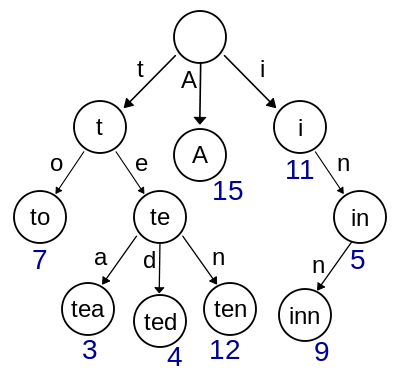
\includegraphics[width=0.33\textwidth]{Trie_example}
    				\caption{A trie for keys "A","to", "tea", "ted", "ten", "i", "in", and "inn"\cite{fig:Trie_example}.}
    				\label{fig:Trie_example}
				\end{wrapfigure}
				
				The trie is a tree like data structure often used for storing strings. Each node in the trie represents a single letter in a string. Each node in a trie has a fixed number of child nodes like a binary search tree. Unlike the binary search tree the trie does not have two child nodes,it has one for each letter of the alphabet. This allows the trie nodes to not store there value because there position determines it. A node's children share a common prefix,that prefix is the value of there parent node.

There are many features of tries that make them a good choice for a predictive text system. One of them is that values can be look up by there prefixes. Predictive text systems use a partial word (a prefix) to search for possible full words. So it's important that prefix lookups are fast and efficient. [TODO:: ADD MORE STUFF HERE]
				
				
			\subsubsection{How I have implemented the trie}
		\subsection{Alternative Data structures}
			\subsubsection{Binary Trees vs Tries}
			
			\subsubsection{Hash map vs Tries}
			\subsubsection{List vs Tries}
	\section{Testing}
		\subsection{Complixity}
			\subsubsection{Time Complexity of Tries}
				The search time for a value in a trie is o(m*c) where m is the length of the word to look up and c is the size of the alphabet. This means that searches in a trie is O(1) which means that the number of items in the trie do not affect the search time. 
				
		\subsection{Unit Testing}
		\subsection{User interactions}
		
	\newpage
	\printbibliography
	\newpage
\end{document}
